\documentclass[a5paper,8pt,twoside]{extarticle}
\usepackage[utf8]{inputenc}
\usepackage[IL2]{fontenc}
\usepackage{geometry}
\usepackage{tikz}
\usepackage{enumitem}
\graphicspath{ {img/} }
\usepackage[czech]{babel}
\usepackage{blindtext}
\usepackage{pifont,mdframed}
\usepackage{fourier}
\usepackage{icomma}
\usepackage{tabularx}
\usepackage[unicode,hidelinks]{hyperref}
\newcommand{\email}[1]{\texttt{\href{mailto:#1}{#1}}}
\newenvironment{warningBox}
  {\par\begin{mdframed}[linewidth=1pt,linecolor=black]%
    \begin{list}{}{\leftmargin=1cm
                   \labelwidth=\leftmargin}\item[\Large\warning]}
  {\end{list}\end{mdframed}\par}
  
  \newenvironment{infoBox}
  {\par\begin{mdframed}[linewidth=1pt,linecolor=black]%
    \begin{list}{}{\leftmargin=1cm
                   \labelwidth=\leftmargin}\item[\Large\lefthand]}
  {\end{list}\end{mdframed}\par}

  \newenvironment{prohibitBox}
  {\par\begin{mdframed}[linewidth=1pt,linecolor=black]%
    \begin{list}{}{\leftmargin=1cm
                   \labelwidth=\leftmargin}\item[\Large\noway]}
  {\end{list}\end{mdframed}\par}

   \newenvironment{function_reference}[1]
   {\par
    \begin{list}{}{\leftmargin=1cm
                   \labelwidth=\leftmargin}\item[{\raisebox{-0.5\baselineskip}{\includegraphics[height=1.5\baselineskip]{#1}}}]}
  {\end{list}\par}

  \newenvironment{function_reference_bodge_trig}[1]
   {\par
    \begin{list}{}{\leftmargin=1cm
                   \labelwidth=\leftmargin}\item[{\raisebox{-3.5\baselineskip}{\includegraphics[height=4.5\baselineskip]{#1}}}]}
  {\end{list}\par}

  \newcommand*\joinBox{\vspace{-0.9em}}
%%%%%%%%%%%%%%%%%%%%%%%%%%%%%%%%%%%%%%%%%%%%%%%%%%%%%%%%%%%%%%%%%%%%%%
% LaTeX Overlay Generator - Annotated Figures v0.0.1
% Created with http://ff.cx/latex-overlay-generator/
% If this generator saves you time, consider donating 5,- EUR! :-)
%%%%%%%%%%%%%%%%%%%%%%%%%%%%%%%%%%%%%%%%%%%%%%%%%%%%%%%%%%%%%%%%%%%%%%
%\annotatedFigureBoxCustom{bottom-left}{top-right}{label}{label-position}{box-color}{label-color}{border-color}{text-color}
\newcommand*\annotatedFigureBoxCustom[8]{\draw[#5,thick,rounded corners] (#1) rectangle (#2);\node at (#4) [fill=#6,thick,shape=circle,draw=#7,inner sep=2pt,font=\sffamily,text=#8] {\textbf{#3}};}
%\annotatedFigureBox{bottom-left}{top-right}{label}{label-position}
\newcommand*\annotatedFigureBox[4]{\annotatedFigureBoxCustom{#1}{#2}{#3}{#4}{red}{white}{black}{black}}
\newcommand*\annotatedFigureText[4]{\node[draw=none, anchor=south west, text=#2, inner sep=0, text width=#3\linewidth,font=\sffamily] at (#1){#4};}
\newenvironment {annotatedFigure}[1]{\begin{tikzpicture}
\node[anchor=south west,inner sep=0] (image) at (0,0) { #1};\begin{scope}[x={(image.south east)},y={(image.north west)}]}{\end{scope}\end{tikzpicture}}
%%%%%%%%%%%%%%%%%%%%%%%%%%%%%%%%%%%%%%%%%%%%%%%%%%%%%%%%%%%%%%%%%%%%%%

\newcommand*\nref[1]{\textbf{(\ref{#1}, str. \pageref{#1})}}
\newcommand*\fref[2]{\textbf{(obr. \ref{#1}#2, str. \pageref{#1})}}
\newcommand*\cleartoleftpage{%
  \clearpage
  \ifodd\value{page}\hbox{}\newpage\fi
}
\title{IVSKalkulátor\\Uživatelský manuál}
\usepackage{}
\author{Lidé u výtahu}
\date{\today}
\begin{document}
    \renewcommand\thesubsubsection{\Alph{subsubsection}}
    \setlength{\parindent}{0em}
    \setlength{\parskip}{1em}
    \begin{titlepage}
        \newgeometry{top=0.75in,bottom=0.75in}
        \begin{center}
            {\LARGE \textsc{Lidé u výtahu}}

            \vspace{\stretch{0.382}}
            {\large Uživatelský manuál}
            
            {\Huge KalkIVSulátor}\\
            \vspace{1.5mm}
            {\huge Pokročilý výpočetní software}\\
            \vspace{\stretch{0.618}}
        \end{center}
        {\large Duben 2020} \hfill {\large Verze 1.0}
    \end{titlepage}
    
    %The following page is the LEFT INSIDE COVER; do not remove this page; keep it blank if need be!
    \thispagestyle{empty}
    \begin{warningBox}
        Skupina Lidé u výtahu se snaží, aby kalkuačka byla pouze co nejpřesnější. Přičemž avšak nemůže garantovat 100\% přesnost a nulovu chybovst výpočtů.

        Používáním kalkulačky souhlasíte, že skupina Lidé u výtahu není zodpovědná za žádnou újmu, materiální či jiného druhu, způsobenou používaní tohoto software.
    \end{warningBox}
    \joinBox
    \begin{warningBox}
        Skupina Lidé u výtahu opovrhuje využívaní tohoto softwaru v akademických kontextech, kde je využívaní kalkulaček zakázáno.

        Skupina Lidé u výtahu nezodpovídá za stanutí před displinární komisí, špatnou známkou či vyloučením plynoucí z používaní tohoto softwaru v nepovelných kontextech.
    \end{warningBox}
    
    \newpage
    \setcounter{page}{1}
    \tableofcontents
    
    \newpage

    \section*{Vítejte}
    Děkujeme za pořízení kalkulačního software od skupiny Lidé~u~výtahu. Jsem si jistí, že náš software Vás nezklame. Ba naopak. Náš software prošel sofistikovaným plánování a vývojem, typické pro inženýry vycházející z nejprestižnějších univerzitních institucí, a zaručejeme Vám stoprocentní spokojenost.

    Potřeba počítat je stará, jako písmo\,--\,mnohé nejstarší dochovalé písemnosti mluví o počtech, o daních. Čísla jsou prostě spjatá s lidskou civilizací. Již staří Egypťané vynalezli abakus\,--\,kuličkové počítadloq\,--\,zařízení pro zjednodušení počtů. A jak se velikost lidských společností zvětšovala, tak i její potřeba pro rychlé a efektivní výpočty. Historie moderních početních zařízení počala roku 1642 vynálezem mechanické kalkulačky Wilhelmem Schickerdem. A jak tato historie postupovala, přes logaritmická pravítka, elektromechanické kalkulátory, počítače založené na relé i tranzistorech, tak se dostala do rukou i nám. S radostí Vám představuje nejnovější eveluce ve světe výpočtů.

    A tímto evoluce nekončí, jak vývoj dnešních technoligií postupuje raketově dopředu, tak postupujeme my: náš software je neustále aktualizován a vyvíjen; jsme odhodlaní přidávat funkce a zůstat na vrcholu výpočetního software.
    
    ---Viktor Rucký, zakladatel skupiny Lidé u výtahu
    \newpage
    \section{Instalace}
    TODO
    \section{Spuštění}
    TODO
    \cleartoleftpage
    \section{Užívání}
    \subsection{Uživatelské rozhraní\,--\,obecné}
    \vfill
    \begin{figure}[h]
        \begin{center}
            \begin{annotatedFigure}
                {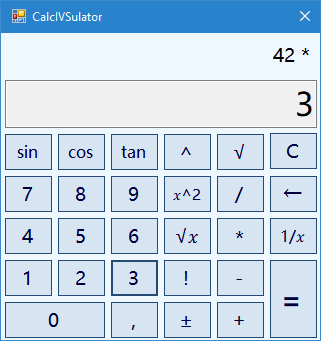
\includegraphics[width=0.75\linewidth]{calculator.PNG}}
                \annotatedFigureBox{0.01,0.0077}{0.9919,0.6176}{A}{0.01,0.31265}%bl
                \annotatedFigureBox{0.01,0.6176}{0.9919,0.7746}{B}{0.01,0.6961}%bl
                \annotatedFigureBox{0.01,0.7746}{0.9919,0.8875}{C}{0.01,0.83105}%bl
                \annotatedFigureBox{0.9,0.9}{1,1}{D}{0.885,0.95}%bl
            \end{annotatedFigure}
        \end{center}
    \caption{Hlavní sekce uživatelského rozhraní}
    \label{fig:UI_main}
    \end{figure}
    \vfill
    \newpage
    Uživatelské rozhraní je tvořeno čtyřmi častmi:

    \subsubsection{Klávesnice}
    Pomocí klávesnice lze zadat data do kalkulačky. Princip operace je vysvětlen v sekci \uv{zadá\-vání čísel} \nref{sec:entering_numbers}. Funkce jednotlivých tlačítek je vysvětlena v sekci \uv{uživatelské rohraní\,--\,klávesnice} \nref{sec:UI_keyboard}.

    \subsubsection{Výsledkový a zadávací displej}
    Zde se zobrazí výsledek Vaši operace nebo právě zadaný operand.

    \subsubsection{Displej s předchozí operací}
    Zde se zobrazí předchozí operand a operace, která je prováděna.

    \subsubsection{Ukončovací křížek}
    Pomocí křížku lze ukončit aplikaci.

    \newpage

    \subsection{Uživatelské rohraní\,--\,klávesnice}
    \label{sec:UI_keyboard}
    \vfill
    \begin{figure}[h]
        \begin{center}
        \begin{annotatedFigure}
            {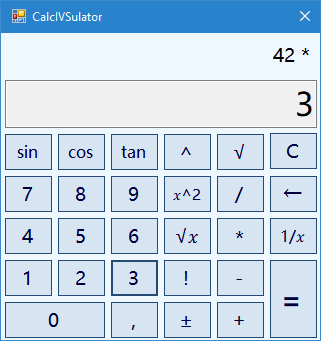
\includegraphics[width=0.75\linewidth]{calculator.PNG}}
            \draw[red, thick, rounded corners] (0.01,0.005) -- (0.335,0.005) -- (0.335, 0.123125) -- (0.5, 0.123125) -- (0.5,0.4925) -- (0.01,0.4925) -- cycle;
            \node at (0.01,0.24875) [fill=white,thick,shape=circle,draw=black,inner sep=2pt,font=\sffamily,text=black] {\textbf{A}};
            \annotatedFigureBox{0.335,0.005}{0.5, 0.123125}{B}{0.4175,-0.01}%bl
            \annotatedFigureBox{0.5,0.005}{0.665, 0.123125}{C}{0.5825,-0.01}%bl
            \annotatedFigureBox{0.83,0.37}{0.9919, 0.4925}{D}{1,0.43125}%bl
            \annotatedFigureBox{0.83,0.4925}{0.9919, 0.615}{E}{1,0.55375}%bl
            \annotatedFigureBox{0.83,0.005}{0.9919, 0.2475}{G}{1,0.12625}%bl
            \draw[green, thick, rounded corners] (0.01,0.4925) -- (0.01,0.615) -- (0.83,0.615) -- (0.83, 0.37) -- (0.9919, 0.37) -- (0.9919,0.2475) -- (0.83,0.2475) -- (0.83,0.005) -- (0.665,0.005) -- (0.665, 0.123125) -- (0.5,0.123125) -- (0.5,0.4925) -- cycle;
            \node at (0.01,0.55375) [fill=white,thick,shape=circle,draw=black,inner sep=2pt,font=\sffamily,text=black] {\textbf{F}};
        \end{annotatedFigure}
      \end{center}
        \caption{Rozdělení klávesnice}
        \label{fig:UI_keyboard}
    \end{figure}
    \vfill
    \newpage
    Klávesnici kalkulačky lze rozdělit do několika funkčních celků.

    \subsubsection{Numerické klávesy}
    Používají se pro zadávání čísel operandů, spolu s klávesami \uv{desetinná čárka} \textbf{(B)} a \uv{změ\-na znaménka} \textbf{(C)}. Viz. sekce \uv{zadávání čísel} \nref{sec:entering_numbers}.

    \subsubsection{Desetinná čárka}
    Pro zadávní desetinné čarky při vkládání čísel. Viz. sekce \uv{zadávání čísel} \nref{sec:entering_numbers}.

    \subsubsection{Změna znaménka}
    Pro změnu znaménka zadaného čísla. Viz. sekce \uv{zadávání čísel} \nref{sec:entering_numbers}.

    \subsubsection{Smazání číslice}
    Smaže poslední číslici (číslici nejnižšího řádu) ve \uv{výsledkovém a zadávacím displeji} \fref{fig:UI_main}{.B}. Viz. sekce \uv{zadávání čísel} \nref{sec:entering_numbers}.

    \subsubsection{Smazat vše}
    Smaže obsah kalkulačky, včetně přechozího čísla a operace. Viz. sekce \uv{obecné používaní} \nref{sec:general_use}.

    \subsubsection{Tlačítka funkcí a operací}
    Tyto tlačítka slouží pro výběr provedené funkce či operace nad zadanými čísly. Viz. sekce \uv{funkce kalkulačky} \nref{sec:function_reference}.

    \subsubsection{Rovná se / potrvrzení}
    Tímto se potvrdí zadané číslo a provede se zadaná binární operace. Viz. sekce \uv{obecné používaní} \nref{sec:general_use}.

    \newpage

    \subsection{Obecné používání}
    \label{sec:general_use}
    Proces pro většinu operací s kalkulačkou je následující. Doporučujeme také přečíst sekci \uv{zadávaní čísel} \nref{sec:entering_numbers}. Jednotlivé funkce a operace kalkulačky jsou popsány v sekci \uv{funkce kalkulačky} \nref{sec:function_reference}.
    \begin{enumerate}
        \item Zadejte číslo prvního operandu pomocí \uv{numerických kláves}, a pokud je třeba, kláves \uv{desetinné čárky} anebo \uv{změny znaménka} \fref{fig:UI_keyboard}{.A/B/C}.
        \item Vyberte požadovaou operaci pomocí \uv{klávesy funkce nebo operace} \fref{fig:UI_keyboard}{.F}.
        \item Pokud je operace unární, zobrazí se výsledek (nebo chybové hlášení) na \uv{vý\-sled\-ko\-vém a zadávacím displeji} \fref{fig:UI_main}{.B}, jinak se zadáný operand a symbol operace zobrazí na \uv{displeji s předchozí operací} \fref{fig:UI_main}{.C}.
        \item Obdobně jako první operand, zadejte druhý operand.
        \item Potvrďte druhý operand pomocí klávesy \uv{rovná se / potrvrzení} \fref{fig:UI_keyboard}{.G}.
        \item Na \uv{výsledkovém a zadávacím displeji} se zobrazí výsledek nebo chybové hlášení; o chybových hlášeních Vás informujeme v sekci \nref{sec:errors}.
    \end{enumerate}
    Pokud jste zadali první operand a vybrali operaci a chcete vybranou operaci změnit, stačí stisknout tlačítko Vaši požadované operace; první operand nebude smazán.

    Pokud jste udělali chybu v zadání prvního operandu, stisknětě klávesu \uv{smazat vše} \fref{fig:UI_keyboard}{.E}; operaci bude třeba opět vybrat.
    \begin{infoBox}
        Kalkulačka používá infixní notaci!
    \end{infoBox}
    \joinBox
    \begin{infoBox}
        Kalkulačka neuplatňuje prioritu operátorů!
    \end{infoBox}
    \joinBox
    \begin{warningBox}
        Kalkulačka se snaží býti velice přesná a má nízkou chybu při výpočtech. Opakované využítí výsledku v operacích způsobuje kumulování chyby, což může snížit přesnost.
    \end{warningBox}
    \subsection{Zadávání čísel}
    \label{sec:entering_numbers}
    Kalkulačka dokáže pracovat s kladnímy celými čísly ale i čísly desetinnímy a zápornými.

    Aktualné zadávané číslo se zobrazí ve \uv{výsledkovém a zadávacím displeji} \fref{fig:UI_main}{.B}.

    Pomocí \uv{numerických kláves} \fref{fig:UI_keyboard}{.A} se zadávají jednotlivé číslice. Vložená číslice se zobrazí na místě jednotek a předchozí číslo se posune o řád doleva, aby vytvořilo místo pro novou číslici (mimo situaci po stisknutí klávesy \uv{desetinná čárka}).

    Pomocí klávesy \uv{desetinná čárka} \fref{fig:UI_keyboard}{.B} se zobrazí desetinná čárka za číslicí řádu jednotek. Nyní se po stiknutí \uv{numerických kláves} nová číslice zobrazí na pravém konci čísla (tj. místě s řádem o jedna menší, než řád již zadané číslice s nejnižším řádem).

    \begin{prohibitBox}
        Opětovné stisknutí klávesy \uv{desetinná čárka} \textbf{nezpůsobí} změnu umístění desetinné čarky! Pomocí klávesy \uv{smazání číslice} je třeba desetinnou čá\-rku nejprve smazat!
    \end{prohibitBox}

    Pokud chcete zadat číslo záporné, použijte klávesu \uv{změna znaménka} \fref{fig:UI_keyboard}{.C}. Opětovné stisknutí klávesy změní zadané číslo zpět na číslo kladné.

    \begin{prohibitBox}
        Nesnažte se zadat záporné číslo pomocí klávesy \uv{odčítání}! Je nutné použít klávesu \uv{změna znaménka}!
    \end{prohibitBox}

    Pokud provedete chybu při zadávání čísla, lze smazat poslední číslici pomocí klávesy \\\uv{sma\-zá\-ní čí\-sli\-ce} \fref{fig:UI_keyboard}{.D}; klávesu lze použít opakovaně. Pokud chcete smazat celé číslo, můžete využít klávesu \uv{smazat vše} \fref{fig:UI_keyboard}{.E}.

    \begin{warningBox}
        Použítí klávesy \uv{smazat vše} také smaže předchozí operand a vybranou operaci.
    \end{warningBox}

    \renewcommand\thesubsubsection{\thesubsection.\arabic{subsubsection}}
    \subsection{Jednotlivé funkce kalkulačky}
    \label{sec:function_reference}
    V této sekci jsou popsány funkce všech \uv{kláves funckí a operací} \fref{fig:UI_keyboard}{.F}.

    \subsubsection{Sčítaní}
    \label{sec:addition}
    \begin{function_reference}{btn_plus}
        Sečte operandy.
    \end{function_reference}
    
    \subsubsection{Odčítaní}
    \label{sec:subtraction}
    \begin{function_reference}{btn_minus}
        Odečte druhý operand od prvního.
    \end{function_reference}

    \subsubsection{Násobení}
    \label{sec:multiply}
    \begin{function_reference}{btn_multiply}
        Vynásobí operandy.
    \end{function_reference}

    \subsubsection{Dělení}
    \label{sec:division}
    \begin{function_reference}{btn_divide}
        Vydělí první operand druhým.
        \begin{infoBox}
            Pro rychlý výpočet obráceného čísla lze využít funkci \uv{obrácené číslo} \nref{sec:inverse}.
        \end{infoBox}
        \joinBox
        \begin{prohibitBox}
            Dělení nulou není definované a způsobí chybové hlášení!
        \end{prohibitBox}
    \end{function_reference}

    \subsubsection{Druhá mocnina}
    \label{sec:square}
    \begin{function_reference}{btn_square}
        Umocní operandu na druhou.
        \begin{infoBox}
            Pro obecnou mocninu použijte funkci \uv{obecná mocnina} \nref{sec:power}.
        \end{infoBox}
    \end{function_reference}

    \subsubsection{(Obecná) mocnina}
    \label{sec:power}
    \begin{function_reference}{btn_power}
        Umocní první operand na druhý. Jsou podporováný i záporné mocniny.
        \begin{infoBox}
            Pro rychlý výpočet druhé mocniny lze využít funkci \uv{druhá mocnina} \nref{sec:square}.
        \end{infoBox}
        \joinBox
        \begin{prohibitBox}
            Druhý operand musí být celé číslo! Jinak se zobrazí chybové hlášení!
        \end{prohibitBox}
        \joinBox
        \begin{prohibitBox}
            Operace $0^0$ není definována a způsobí chybové hlášení!
        \end{prohibitBox}
    \end{function_reference}

    \subsubsection{(Druhá) odmocnina}
    \label{sec:sqrt}
    \begin{function_reference}{btn_sqrt}
        Vypočítá druhou odmocninu zadaného čísla.
        \begin{infoBox}
            Pro obecnou odmocninu využijte funkci \uv{obecná mocnina}\\ \nref{sec:root}.
        \end{infoBox}
        \joinBox{}
        \begin{prohibitBox}
            Kalkulačka nepodporuje komplexní odmocninu!\\
            Odmocnina záporných čísel není definována a způsobí chybové hlášení!
        \end{prohibitBox}
    \end{function_reference}

    \subsubsection{Obecná odmocnina}
    \label{sec:root}
    \begin{function_reference}{btn_root}
        Odmocní první operand řádem druhého operandu.
        \begin{infoBox}
            Pro rychlý výpočet druhé odmocniny lze využít funkci \uv{druhá odmocnina} \nref{sec:sqrt}.
        \end{infoBox}
        \joinBox
        \begin{prohibitBox}
            Kalkulačka nepodporuje komplexní odmocninu!\\
            Odmocnina záporných čísel se sudým odmocněncem není definována a způsobí chybové hlášení!
        \end{prohibitBox}
        \joinBox
        \begin{prohibitBox}
            Odmocnění nuly se záporným řádem není definována a způsobí chybové hlášení!
        \end{prohibitBox}
        \joinBox
        \begin{prohibitBox}
            Odmocnina nultého řádu není definována a způsobí chybové hlášení!
        \end{prohibitBox}
    \end{function_reference}

    \subsubsection{Faktoriál}
    \label{sec:factorial}
    \begin{function_reference}{btn_factorial}
        Vypočítá faktoriál operandu.
        \begin{infoBox}
            Nejvyšší možný faktoriál je $170!$.
        \end{infoBox}
        \joinBox
        \begin{prohibitBox}
            Faktoriál záporných a desetinných čísel není definovaný a způsobí chybové hlašení!
        \end{prohibitBox}
    \end{function_reference}

    \subsubsection{Goniometrické funkce}
    \label{sec:trig}
    \begin{function_reference_bodge_trig}{btn_trig}
        Vypočítá vybranou goniometrickou funkci\,--\,sinus, kosinus, nebo tangens. Úhel

        \vspace{-4.5em} je zadaný v radiánech.
        \begin{warningBox}
            Je třeba zadat argument goniometrických funkcí v radiánech.
        \end{warningBox}
        \joinBox
        \begin{prohibitBox}
            Tangens $(2k+1)\pi, k \in \mathbb{Z} $ není definovaný a způsobí chybové hlášení.
        \end{prohibitBox}
    \end{function_reference_bodge_trig}

    \subsubsection{Obrácené číslo}
    \label{sec:inverse}
    \begin{function_reference}{btn_inverse}
        Vypočíta obrácené číslo operandu.
        \begin{infoBox}
            Tato operance je ekvivalentní k operaci $1 / X$ \nref{sec:division}.
        \end{infoBox}
        \joinBox
        \begin{prohibitBox}
            Obrácené číslo nuly není definované a způsobí chybové hlášení.
        \end{prohibitBox}
    \end{function_reference}

    \subsection{Chybová hlášení}
    \label{sec:errors}

    Při operaci kalkulačky mohou nastat chybová hlášení.

    \subsubsection{\texttt{No input given}}
    Nezadal jste žádný operand.

    \subsubsection{\texttt{Overflow chyba}}
    Požadovaná operace vrátilo číslo mimo kalkulační rozsah kalkulátoru.

    \subsubsection{\texttt{Dělení nulou}}
    Dělíte nulou nebo se pokušíte provést operaci, která interně se o dělení nulou snaží.

    Podívejte se na nedefinované hodnoty funkce, kterou se snažíte použít v sekci \uv{jednotlivé funkce kalkualčky} \nref{sec:function_reference}.

    \subsubsection{\texttt{Nepovolená operace}}
    Snažíte se provést operaci se vstupem, který není platný.

    Podívejte se na nedefinované hodnoty funkce, kterou se snažíte použít v sekci \uv{jednotlivé funkce kalkualčky} \nref{sec:function_reference}.    

    \section{Technické informace}

    \begin{table}[h]
    \begin{tabular}{|p{19em}|p{19em}|}
    \hline
    Počet číslic využívaných při vnitřních výpočtech & 15 \\ \hline
    Přesnost & 10 desetinných míst (chyba se kumuluje při opakovaných operací s výsledkem) \\ \hline
    Maximální hodnota & $1,7976931348623157 \cdot 10^{308}$ \\ \hline
    Minimální hodnota & $-1,7976931348623157 \cdot 10^{308}$ \\ \hline
    \end{tabular}
    \end{table}

    \section{Autoři}

    Program KalkIVSulátor je autorským dílem skupiny Lidé u výtáhu, která je tvořena těmito lidmi:

    \begin{itemize}
        \item Ondřej Sloup (\email{xsloup02@stud.fit.vutr.cz})
        \item Viktor Rucký (\email{xrucky01@stud.fit.vutr.cz})
        \item Vojtěch Vlach (\email{xvlach22@stud.fit.vutr.cz})
    \end{itemize}

    \begin{infoBox}
        Viktor Rucký sbírá pohlednice. Pokud chcete, napište Viktorovi o poštovní adresu e-mailem a pošlete mu pohlednici!
    \end{infoBox}

    \begin{tabularx}{\textwidth}{X X}
        \raisebox{-5em}{
\includegraphics[scale=0.25]{logo_fit.pdf}} & Tento software byl vyvinut jako projekt předmětu IVS studenty Fakulty informačních technoligií Vysokéhu učení technického v Brně.
    \end{tabularx}
    \section{Licence a právní náležitosti}

    Tento program je šířen pod licencí \texttt{GNU GPL v. 3}.

    %The following page is THE BACK COVER; do not remove the page; leave the page blank if need be.
    \cleartoleftpage
    \newgeometry{top=0.75in,bottom=0.75in}
    \thispagestyle{empty}
    \null
    \vfill
    {\large \textsc{Lidé u výtahu}}
\end{document}
